\chapter{Introduction}

\section{Preamble}

\subsection{Cancer epidemiology}

Cancer is a leading cause of death worldwide, accounting for nearly
10 million deaths in 2020 \cite{ferlay_cancer_2021}. The most common new cases
of cancer in 2020 were:
breast cancer, with 2.26 million cases;
lung cancer, with 2.21 million cases;
colon and rectum cancers, with 1.93 million cases;
prostate cancer, with 1.41 million cases;
skin cancer (non-melanoma), with 1.20 million cases;
and stomach cancer, with 1.09 million cases.
The most common causes of cancer death in 2020 were:
lung cancer, with 1.80 million deaths;
colon and rectum cancers, with 916,000 deaths;
liver cancer, with 830,000 deaths;
stomach cancer, with 769,000 deaths;
and breast cancer with 685,000 deaths.
Each year, approximately 400,000 children develop cancer. The most common
cancers vary between countries, but cervical cancer is the most common in 23
countries.

\begin{figure}[h]
    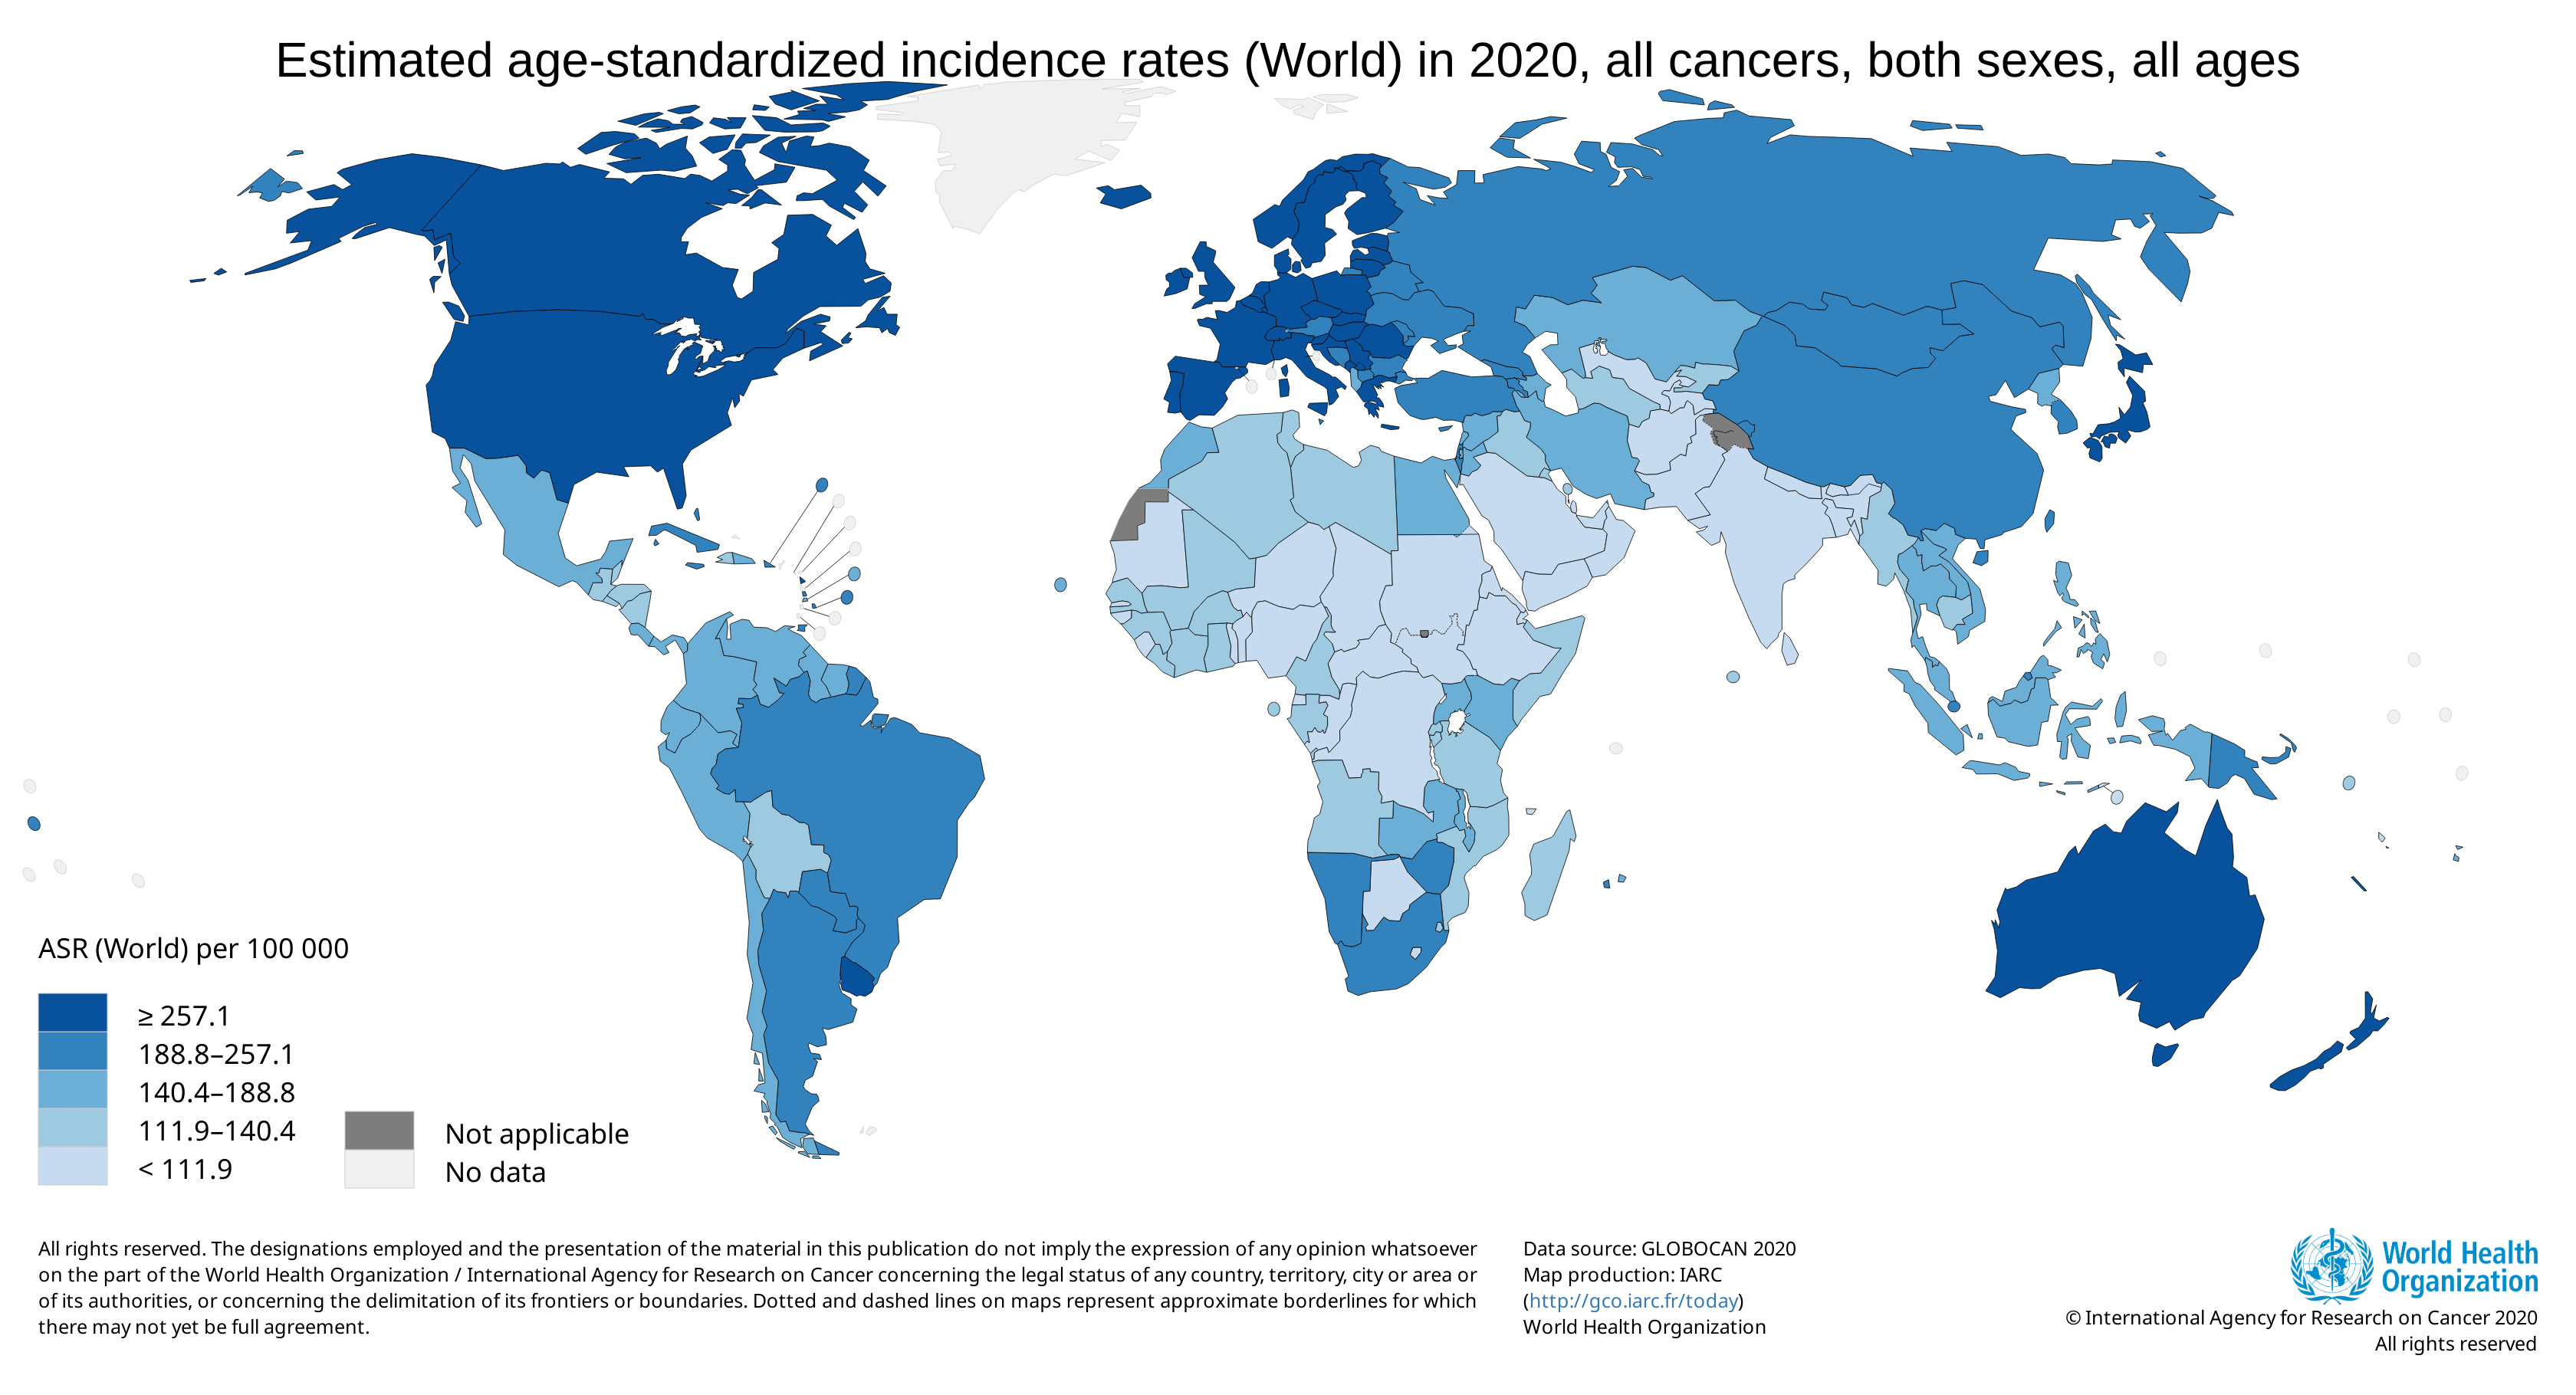
\includegraphics[width=1\textwidth]{images/intro/cancer-asr-world.png}
    \centering
    \caption{ \textbf{Cancer epidemiology.} Bla. }
    \label{fig:cancer-asr}
\end{figure}

\begin{figure}[h]
    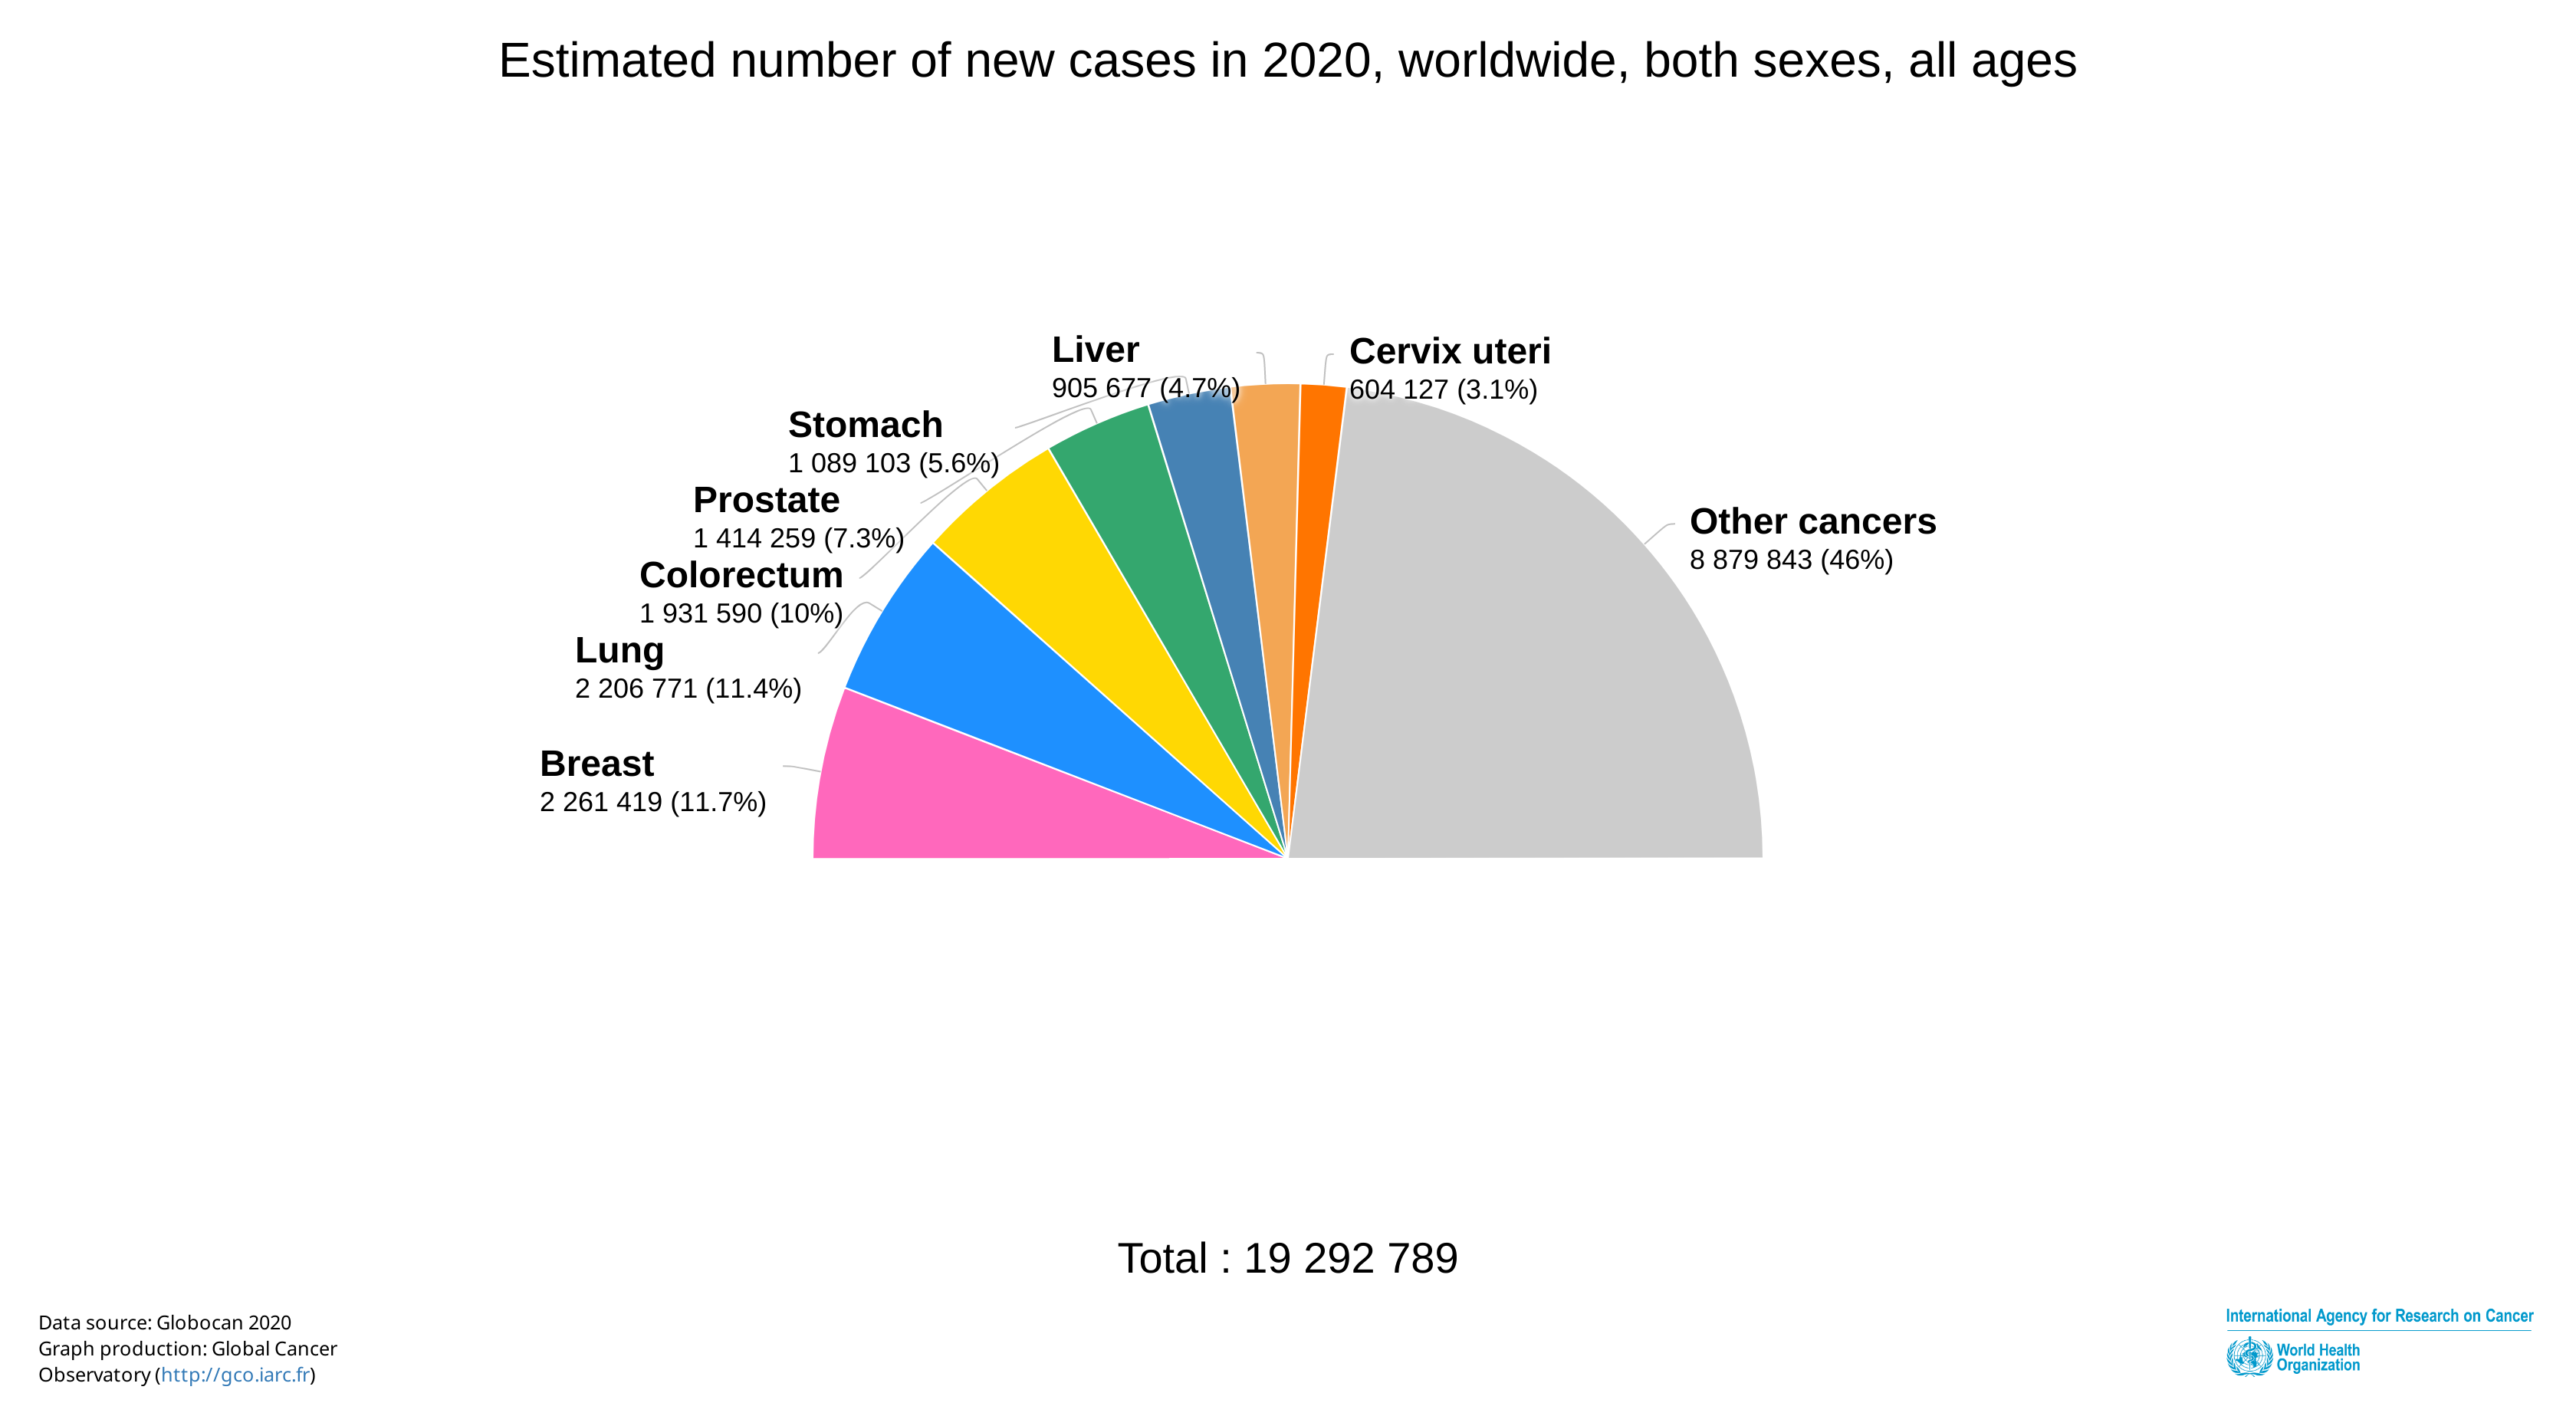
\includegraphics[width=1\textwidth]{images/intro/cancer-proportion.png}
    \centering
    \caption{ \textbf{Cancer epidemiology.} Bla. }
    \label{fig:cancer-proportion}
\end{figure}

\begin{figure}[h]
    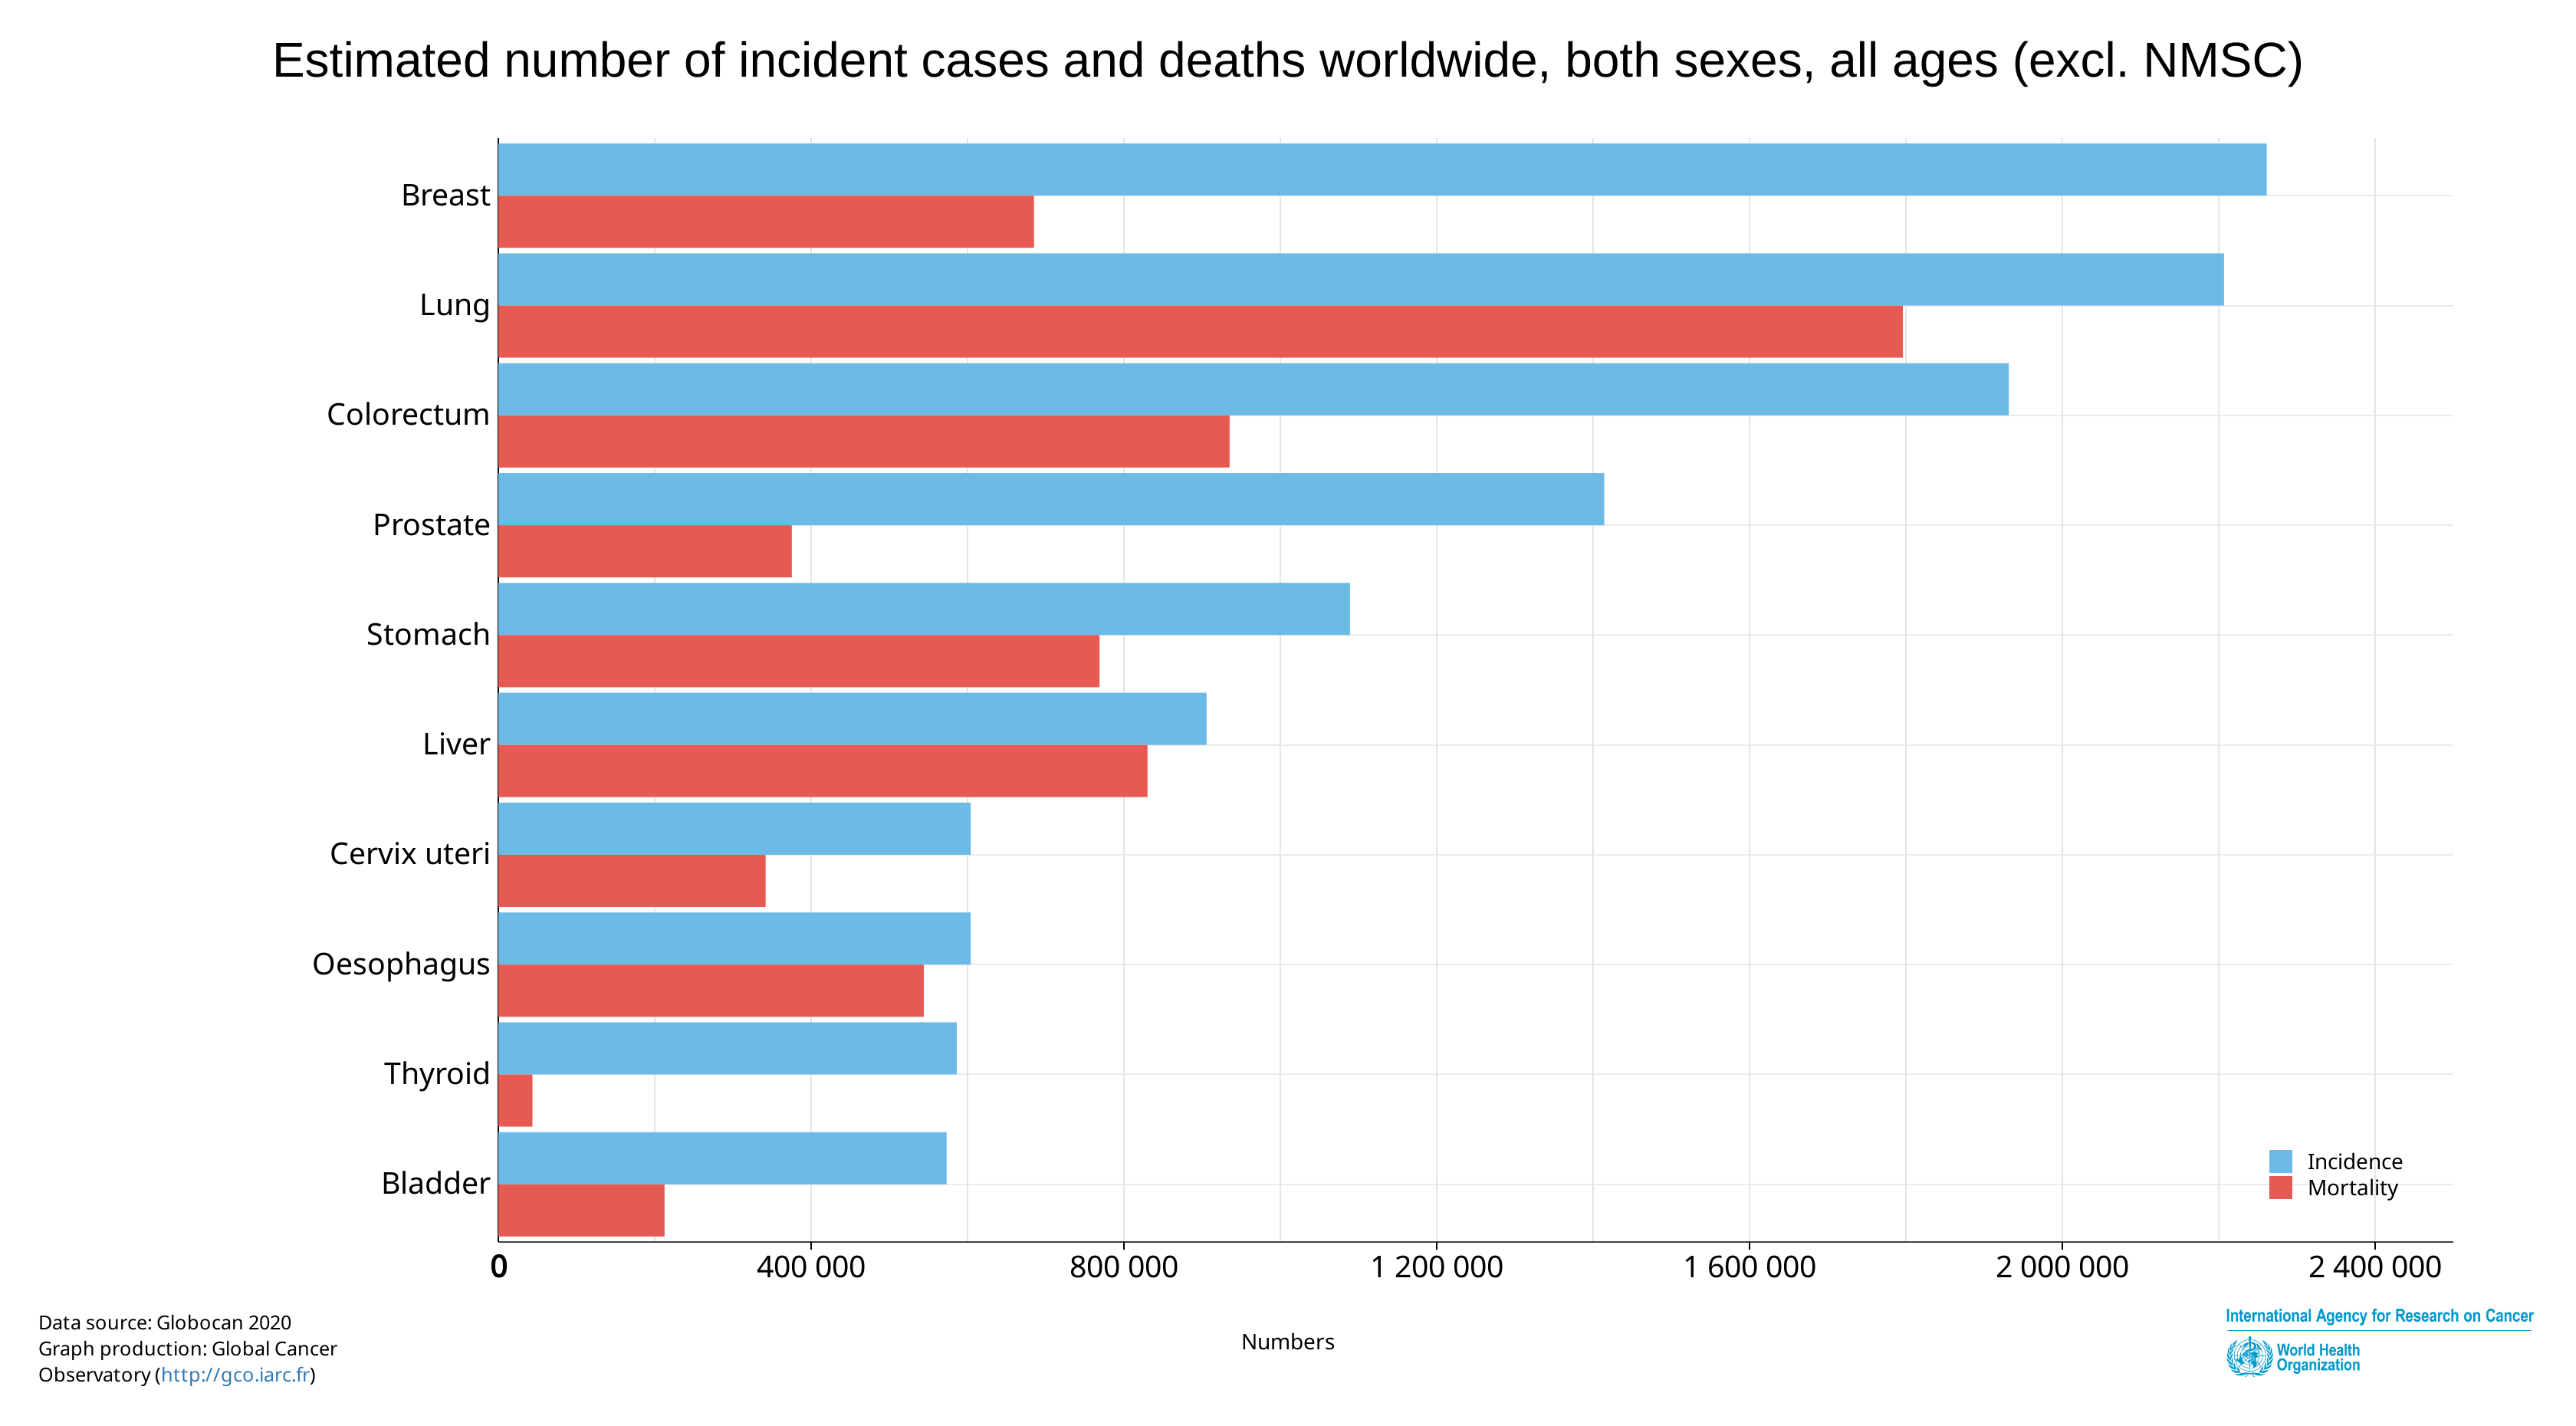
\includegraphics[width=1\textwidth]{images/intro/cancer-incidence-mortality.png}
    \centering
    \caption{ \textbf{Cancer epidemiology.} Bla. }
    \label{fig:cancer-epidemio}
\end{figure}


\subsection{What causes cancer}

Cancer arises from the transformation of normal cells into tumour cells in a
multi-stage process that generally progresses from a pre-cancerous lesion to a
malignant tumour. These changes are the result of the interaction between a
person's genetic factors and three categories of external agents, including:
physical carcinogens, such as ultraviolet and ionizing radiation; chemical
carcinogens, such as asbestos, components of tobacco smoke, alcohol, aflatoxin
(a food contaminant), and arsenic (a drinking water contaminant); and biological
carcinogens, such as infections from certain viruses, bacteria, or parasites.
The incidence of cancer rises dramatically with age, most likely due to a
build-up of risks for specific cancers that increase with age. The overall risk
accumulation is combined with the tendency for cellular repair mechanisms to be
less effective as a person grows older.

\subsection{Risk factors}

Tobacco use, alcohol consumption, unhealthy diet, physical inactivity and air
pollution are risk factors for cancer and other noncommunicable diseases.  Some
chronic infections are risk factors for cancer; this is a particular issue in
low and middle-income countries. Approximately 13\% of cancers diagnosed in 2018
globally were attributed to carcinogenic infections, including Helicobacter
pylori, human papillomavirus (HPV), hepatitis B virus, hepatitis C virus, and
Epstein-Barr virus (2). Hepatitis B and C viruses and some types of HPV increase
the risk for liver and cervical cancer, respectively. Infection with HIV
increases the risk of developing cervical cancer six-fold and substantially
increases the risk of developing select other cancers such as Kaposi sarcoma.

\subsection{Reducing the cancer burden}

Between 30 and 50\% of cancers can currently be prevented by avoiding risk
factors and implementing existing evidence-based prevention strategies. The
cancer burden can also be reduced through early detection of cancer and
appropriate treatment and care of patients who develop cancer. Many cancers have
a high chance of cure if diagnosed early and treated appropriately.

Cancer risk can be reduced by: not using tobacco; maintaining a healthy body
weight; eating a healthy diet, including fruit and vegetables; doing physical
activity on a regular basis; avoiding or reducing consumption of alcohol;
getting vaccinated against HPV and hepatitis B if you belong to a group for
which vaccination is recommended; avoiding ultraviolet radiation exposure (which
primarily results from exposure to the sun and artificial tanning devices)
and/or using sun protection measures; ensuring safe and appropriate use of
radiation in health care (for diagnostic and therapeutic purposes); minimizing
occupational exposure to ionizing radiation; and reducing exposure to outdoor
air pollution and indoor air pollution, including radon (a radioactive gas
produced from the natural decay of uranium, which can accumulate in buildings —
homes, schools and workplaces).

Cancer mortality is reduced when cases are detected and treated early. There are
two components of early detection: early diagnosis and screening. When
identified early, cancer is more likely to respond to treatment and can result
in a greater probability of survival with less morbidity, as well as less
expensive treatment. Significant improvements can be made in the lives of cancer
patients by detecting cancer early and avoiding delays in care. Screening aims
to identify individuals with findings suggestive of a specific cancer or
pre-cancer before they have developed symptoms. When abnormalities are
identified during screening, further tests to establish a definitive diagnosis
should follow, as should referral for treatment if cancer is proven to be
present.

\subsection{Cancer treatment}
A correct cancer diagnosis is essential for appropriate and effective treatment
because every cancer type requires a specific treatment regimen. Treatment
usually includes surgery, radiotherapy, and/or systemic therapy (chemotherapy,
hormonal treatments, targeted biological therapies). Proper selection of a
treatment regimen takes into consideration both the cancer and the individual
being treated. Completion of the treatment protocol in a defined period of time
is important to achieve the predicted therapeutic result. Determining the goals
of treatment is an important first step. The primary goal is generally to cure
cancer or to considerably prolong life. Improving the patient's quality of life
is also an important goal. This can be achieved by support for the patient's
physical, psychosocial and spiritual well-being and palliative care in terminal
stages of cancer. Some of the most common cancer types, such as breast cancer,
cervical cancer, oral cancer, and colorectal cancer, have high cure
probabilities when detected early and treated according to best practices.

\section{Subject definition}

\subsection{Care pathways}

The French Cancer Plan \cite{buzyn_plan_2014} 2014-2019 announces the objectives
to be implemented in the fight against cancer in France. In particular,
objectives 2 and 7 insist on the quality of the care pathway: they aim
respectively to ``guarantee the quality and safety of care'' and ``ensure
comprehensive and personalized care''. In order to standardize the care pathway
while personalizing management, care trajectories have been established. The
definition of these optimal care trajectories is based on national and
international good practice recommendations.

\ac{inca} has published several studies comparing care pathways in France with
national and international recommendations. One of them concerns the time
required for the management of breast and lung cancer. This study found
differences according to the status of the institution of first therapeutic
management or the region \cite{bernard_ledesert_etude_2012}. However, the study
does not explain these differences, in particular because of the lack of
availability of socio-demographic indicators. Today, there are several public
data sources that provide access to these indicators at the municipality level.
Incorporating additional data sources could lead to better understanding of
where these disparities in management come from according to the care
facilities. Indeed, the multiplicity of care centers, their types, the distance
of the care centers from the patients' homes and the location of treatments are
all factors that can degrade the care pathway and impact the prognosis of cancer
patients.

\subsection{Evidences of disparities}

\subsubsection{Geographical disparities}

A study analyzed the care pathways in Tanzania for patients with tuberculosis
\cite{mhalu_pathways_2019}. The study highlights the complexity of the pathways
from the first symptoms to diagnosis and the high cost of accessing health care
facilities. Several studies have investigated the optimal distribution of care
centers in different countries, as well as their accessibility by road or public
transport. A study of health care facilities for the city of Shenzhen in China
showed differences in access to health care depending on the mode of transport
used. It appears that public transport users are at a disadvantage compared to
patients with a car \cite{tao_spatial_2018}. Mandel et al
\cite{mandel_optimizing_2018} showed that an application similar to Google Maps
for guiding patients to different care centers in a multi-site hospital reduces
patient travel time. In particular, the application uses real-time traffic data
for referral. Jia et al \cite{jia_selecting_2014} proposed a method to select
the optimal care center using several criteria such as geographic accessibility
and service quality. In particular, transportation networks such as high-speed
lines and highways are taken into account in the center selection.

\subsubsection{Socio-demographic disparities}

Various studies have investigated the impact of socio-demographic factors on the
course of care and survival prognosis of patients. An American study on lung
cancer patients showed that good physical and intellectual conditions were
linked to better survival from the disease
\cite{pierzynski_socio-demographic_2018}. A second study shows differences in
access to care related to ethnicity for patients with psychosis
\cite{anderson_meta-analysis_2014}. Even though the burden of cancer is easing
in the United States, the decline is unequal among different racial, ethnic and
socio-economic groups \cite{viswanath_science_2005}. The aim of this study was
to examine the impact of patient demographics, tumor characteristics, and
treatment type on time to treatment (TTT) in patients with breast cancer treated
at a safety net medical center with a diverse patient population. Longer median
TTT was noted for Black and single patients \cite{khanna_impact_2017}.

\subsubsection{Gender-related disparities}

Gender appears to have an impact on care pathways. For example, men may have
difficulty talking about their symptoms, fearing that it will be perceived as a
sign of weakness; whereas women who require care are more likely to be neglected
\cite{ferrari_gender_2018}. Indeed, women with myocardial infarction have a
higher mortality rate than men, and this discrepancy appears to be partially due
to delayed diagnosis and access to appropriate care
\cite{bugiardini_delayed_2017}. Similarly, a pediatric study of kidney
transplantation showed that young girls had less rapid access to transplantation
than young boys. This is partly due to non-medical reasons such as parental and
practitioner behavior regarding organ donation \cite{hogan_j_gender_2016}. More
specifically, the gender of the patient could have an impact on the oncology
care pathway. Indeed, several studies show that women's treatment for several
types of cancers is suboptimal. This would at least partially explain why their
chances of survival from these diseases are lower than those of men
\cite{park_a_undertreatment_2019,carter_paulson_e_gender_2009,rose_sex_2016}.
The above examples suggest that patient survival could be improved by taking
gender into consideration in the care pathway. However, at present, gender
differences in the oncology care pathway are barely explored.

\section{Hypothesis and objectives}

\section{Organization and contributions of the thesis}

\subsection{Thesis chapters}

\subsubsection{Care center characterization}
In this chapter, we first proposed a method to automatically label
all the hospitals in metropolitan France, based on their statistics and
available health services. Lastly, we studied the collaborations between
the hospitals, based on patients who visited multiple hospitals during their
pathways. Through community detection algorithms, we grouped hospitals that
frequently exchange patients together. By adding the oncology specialization
label within the discovered communities, we believe we can propose new
hospital groups that are based on patient real-life data, to improve
collaborations and ultimately benefit the patients.

\subsubsection{Accessibility score}
In what follows, we applied \ac{sa} methods to
quantify the accessibility the oncology care in metropolitan France.
Intuitively, we compute a score for every municipality that measures how easy it
would be for patients living in a given municipality to reach oncology care.

\subsubsection{Accessibility optimization}
In this work, we are interested in the case where the health facilities locations are
fixed, and the only lever to improve accessibility is to increase their
capacities.Given a capacity budget, we want to know which facilities to grow and
by how much. We introduce \ac{camion}, an accessibility optimization algorithm
based on \ac{fca} and \ac{lp}. The initial accessibility score was computed with
the \ac{e2sfca} algorithm \cite{luo_enhanced_2009} but our algorithm can
generalize to more \ac{fca} derivatives. In the following sections, we proposed
two approaches for optimizing the accessibility scores. The first one is an
overall optimization, where we seek to maximize the total accessibility. The
second one is a maxi-min optimization, where we want to maximize the minimum
accessibility instead. The first approach could be seen as efficiency
maximization where the second method aims towards equity. Then, we embedded our
results and algorithms into a web application  called
``oncology-accessibility''. Through this web application, we let the users run
the optimization algorithm with the parameters they want, and visualize the
output on interactive maps and figures. We believe such an app could benefit the
healthcare professionals, to help addressing the accessibility disparities in
the country.

\subsubsection{Patients routes}
In this chapter, we analyzed the travels of cancer patients in metropolitan
France. Our goal was to assess whether the earlier observations on the negative
effects of centralization of care were happening in France. Hence, we first
described the travel duration distribution in metropolitan France, and compared
it with the population densities and the oncology specialization of the visited
hospital. Then, we argued that the negative effects of travel on cancer patients
was not only due to driving distance and duration: the road sinuosity should
also be taken into account. We proposed a travel burden index, which is a
composite indicator based on multiple variables to evaluate how easy it is to go
from a population location to an hospital. Additionally, we estimated the carbon
footprint of cancer patients travels, and compared these numbers across the
different regions. Finally, we ran an optimization algorithm to simulate the
scenario where every patient traveled to the closest hospital, such that the
hospitals capacities were not exceeded. We only considered Breast Cancer
patients as this cancer is relatively frequent, and many hospitals have the
required expertise.

\subsubsection{Transparent healthcare}
With these evidences of healthcare information needs, we developed Healthcare
Network, a web application that lists every hospital in France, and displays key
statistics on them. The application is directed to either health professionals
or patients. Health professionals might use it to gain insights about specific
hospitals, and look for the best place to send their patients when they lack
expertise. Patients could learn more about the hospital they have been sent to,
check the care quality or surgery volume.

\subsection{Articles and preprints}
